\hypertarget{grand-uxe9cart-entre-tradition-et-gratte-ciels.}{%
\section{Grand-écart entre tradition et
gratte-ciels.}\label{grand-uxe9cart-entre-tradition-et-gratte-ciels.}}

Après notre sympathique escapade méridionale, et même si Flo l'a déjà
arpentée en long en large et en travers, nous sommes allés nous
installer à Tokyo. Chez Boris et Miwa plus exactement, qui nous ont
généreusement ouvert leurs portes dans le quartier du Tokyo Dome. Nous
avons récupéré en chemin ma cousine canadienne Marianne, qui est venue
partager un bout de vacances avec nous !

\begin{figure}
\centering
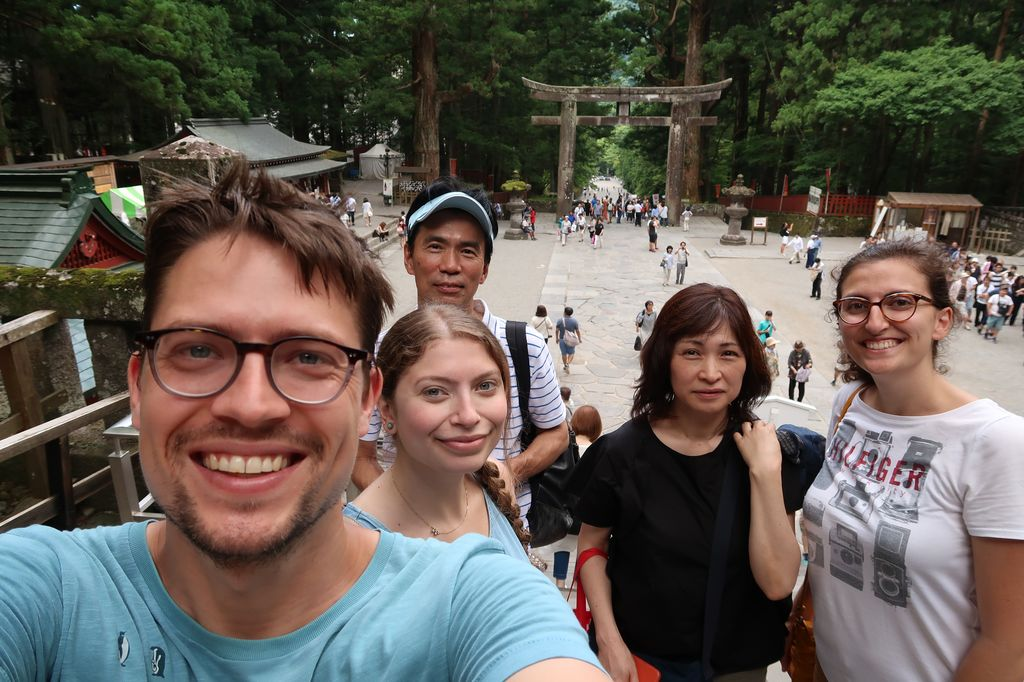
\includegraphics{images/20180710_nikko.JPG}
\caption{Excursion à Nikko avec Masaru et Keiko.}
\end{figure}

Mais après une soirée sous la chaleur de la capitale, nous voilà à
nouveau dans le train : Masaru, un ami de Flo, nous a concocté un
programme plein de surprises et de tradition pour le weekend. On le
retrouve à Mito, puis il nous fait passer par Oarai, ville de bord de
mer équipée d'un centre de recherche où Flo a passé une grosse partie de
sa seconde année au Japon. Après une très agréable soirée chez lui en
compagnie de Keiko, sa femme, nous partons le lendemain pour Nikko. On y
visite un sanctuaire impressionnant, le lac de Chuzenji, et en milieu
d'après-midi on s'installe dans un ryokan (hôtel traditionnel) pour
profiter des onsen (bains chauds) venant des sources volcaniques
avoisinantes. Pour ceux qui sont curieux il y a plein d'explications sur
le "rituel du onsen" partout sur internet, mais sachez que se baigner
dans son plus simple appareil dans des bassins fumants est très relaxant
et agréable, une fois passée l'appréhension initiale de laisser son
maillot de bain dans son sac ! Et le dîner gargantuesque qui suit la
baignade ne gâche aucunement le plaisir...

\begin{figure}
\centering
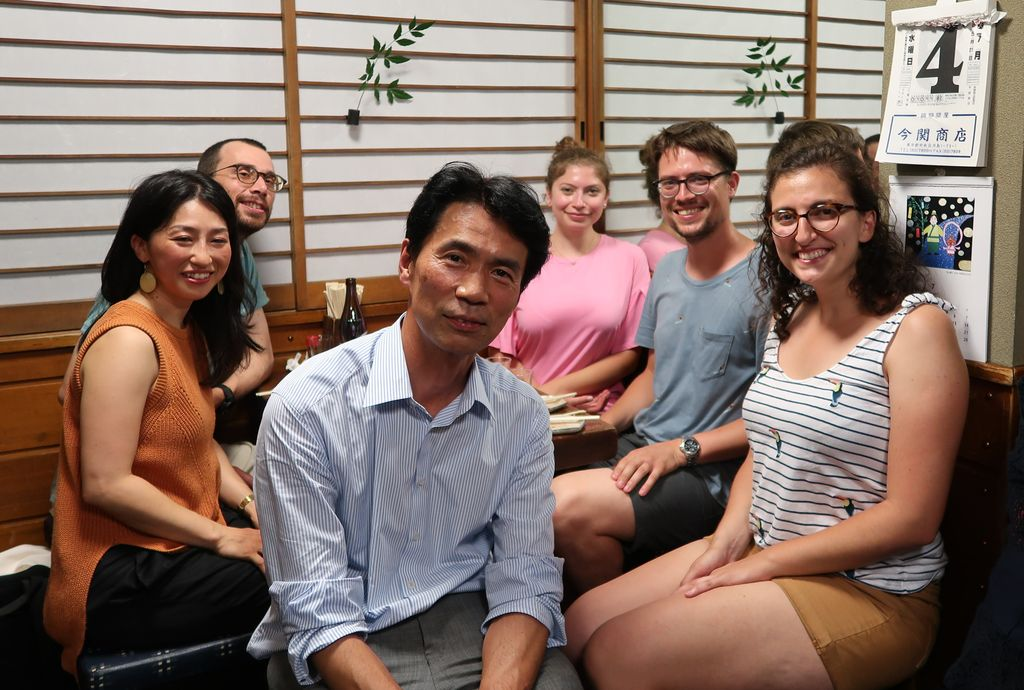
\includegraphics{images/20180710_boris.JPG}
\caption{Excellente soirée ponctuée de découvertes gustatives avec
Boris, Miwa et Masaru à Ginza.}
\end{figure}

De retour à Tokyo, on a arpenté les différents quartiers : Asakusa et
son temple, Ueno et son parc aux multiples musées, Harajuku et ses
magasins, Shinjuku et ses buildings imposants, la vibrante Shibuya, et
complètement à l'opposé le calme quartier de Yanaka et son immense
cimetière. Tout ce que mon imagination avait projeté sur cette ville, je
l'ai retrouvé. Modernité et tradition, j'ai l'impression qu'on se répète
mais c'est vraiment le ressenti que j'en garde. Modernité par l'aspect,
l'architecture, l'activité incessante, ces salarymen en chemise blanche
qui grouillent du matin au soir. Tradition par le caractère des gens,
les rapports extrêmement respectueux, les nombreux temples et
sanctuaires, et bien sûr la nourriture !

\begin{figure}
\centering
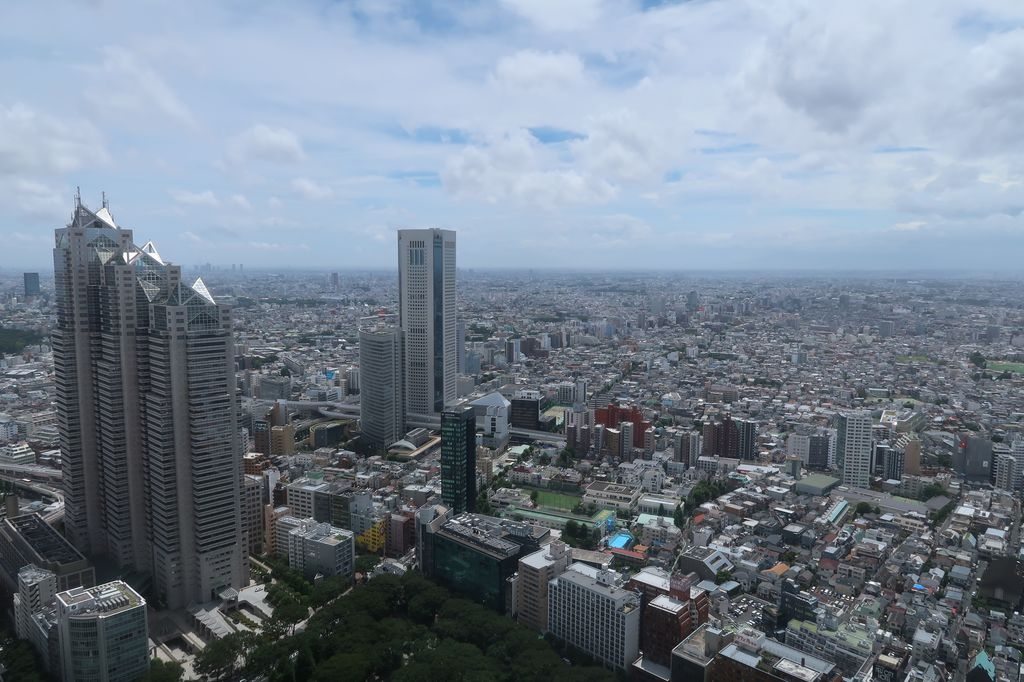
\includegraphics{images/20180710_shinjuku.JPG}
\caption{Tokyo vue d'en haut depuis le siège de la métropole à
Shinjuku.}
\end{figure}

Le temps d'une journée, nous avons aussi découvert la ville de Kamakura,
avec son grand Bouddha de bronze et le magnifique sanctuaire Hasedera.
On a même fini par une baignade dans les eaux tièdes mais agitées de
l'océan !

Notre prochaine étape nous mène à Kyoto, l'ancienne capitale. À suivre !

\emph{Elida et Florian}
